\section{Driedimensionale stapelproblemen}
In de voorbije lessen, hielden we ons bezig om cirkels op een zo optimaal mogelijke manier te stapelen in een driehoek, rechthoek, cirkel ...
Als we dit probleem veralgemenen naar het driedimensionaalgeval, dan krijgen we het zogenaamde probleem van Kepler.

\subsection{Kanonskogels stapelen}

\begin{wrapfigure}[10]{r}{0.3\textwidth}
  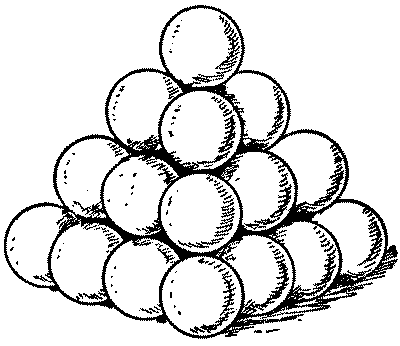
\includegraphics[width=0.3\textwidth]{cannonballs}
\end{wrapfigure}

Ondanks dat het bolstapelprobleem ook het probleem van Kepler genoemd wordt, ontstond het niet bij Kepler, maar bij de Engelse admiraal Sir Walter Raleigh. Wanneer deze Engelse admiraal naar buiten keek vanuit zijn admiraliteitsgebouw, zag hij steeds piramidevormige stapels bestaande uit kanonskogels.  Deze stapels intrigeerden hem zodanig, dat hij zich op een welbepaalde dag afvroeg hoeveel kanonskogels er in zo'n stapel aanwezig waren. Daarom ging hij ten rade bij zijn wetenschappelijk adviseur, Thomas Harriot, om dit  raadsel voor hem op te lossen. 

Voor deze les gaan we ons wat inleven in de rol van Sir Walter Raleigh. Alleen zullen we nu het niet direct vragen aan Thomas Harriot, maar het zelf onderzoeken.

Bolvormige kanonskogels kun je op verschillende manieren als een piramide op elkaar stapelen. Je kunt bijvoorbeeld beginnen om de eerste laag kogels in een vierkant patroon te leggen, maar ook volgens gelijkzijdige driehoeken is het mogelijk, net als bij de jetons in het vlak of de blikjes/glazen op het dienblad. 
Omdat we toevallig niet voldoende kanonskogels bij de hand hebben, kunnen we knikkers gebruiken om dit uit te proberen (ook tafeltennisballetjes of sinaasappelen zijn geschikt).

\todo{Uitgangspunt cursus}
Het is nu de bedoeling dat de leerlingen zelf de formule gaan zoeken en vinden door dit uit te testen voor verschillende vormen van grondvlakken en voor verschillende lagen ($n = 1, 2, ... , 6 , ... , 100$).
\begin{itemize}
	\item Vierkant grondvlak
	\item Driehoekig grondvlak
	\item Zeshoekig grondvlak
	\item Cirkelvormig grondvlak
\end{itemize}
\question{We zien wel wat haalbaar is. Ook voor ons om een formule te vinden ...
De knikkers lijken mij het handigste, alleen weet ik eigenlijk niet hoe die best blijven liggen, want gewoon op tafel rollen die natuurlijk weg en kan je bijvoorbeeld nooit 6 lagen deftig krijgen.}

\todo{Uitgangspunt cursus}
De leerlingen zullen algauw gevonden hebben hoeveel knikkers ze moeten gebruiken voor de verschillende rijen.
\newpage

\begin{table}
\centering
\begin{tabular}{l|c|c|c|c|c|c}
Aantal lagen: &1&2&3&4&5&6\\\hline\hline
Driehoek: &1&4&10&20&35&56 \\\hline
Vierkant: &1&5&14&30&55&91 \\\hline
Zeshoek: &&&&&&\\\hline
Cirkel:&&&&&&
\end{tabular}
\caption{Aantal knikkers voor verschillende piramides met $n$ lagen}
\end{table}

\todo{Uitgangspunt cursus}
Ook de formule met de sommen moet zeker mogelijk zijn om gevonden te worden.

\begin{itemize}
	\item Formule bij piramide met driehoekig grondvlak:
	 $$d(n)= \frac{1.2}{2} + \frac{2.3}{2}+\frac{3.4}{2} + \cdots + \frac{n(n+1)}{2}$$
	\item Formule bij piramide mert vierkant grondvlak: $$v(n)=1^2 + 2^2 + \cdots + n^2$$
\end{itemize}

Ook kunnen we de leerlingen andere zaken laten onderzoeken met deze knikkers:
\begin{itemize}
	\item Kan je van twee vierkante piramides een nieuwe vierkante piramide maken? Of beter geformuleerd: denk je dat ... vermoed je dat ...
	\item Kan je van twee driehoekige piramides een nieuwe driehoekige piramide maken?
	\item Kan je van een combinatie van driehoekige en vierkante piramides een vierkante piramide maken?\\
Opmerking: piramides van ��n verdiep hoog worden niet meegerekend ;).
\end{itemize}

Na deze testfase is het de bedoeling dat we dit klassikaal overlopen.


\subsubsection{Het aantal kanonskogels bij een piramide met vierkant grondvlak}

\todo{De volgende alinea vind ik een goede manier om te schrijven. Gebruik van 'We' en 'Je' en niet zoals voordien gebruik van 'De leerlingen'}

We zullen beginnen met de vierkante stapeling.
Om bijvoorbeeld een stapel van vier lagen hoog te maken begin je om 16 kogels netjes in een 4 bij 4 vierkant te leggen. Vervolgens leg je daarop een laag van 9 kogels in een 3 bij 3 vierkant, dan een laag met $2\times2=4$ kogels, en ten slotte is er nog plaats voor ��n kogel als top van de piramide. Voor een 'vierkante' stapel van vier lagen hoog heb je dus $16+9+4+1=30$ kogels nodig.
Als we kijken naar de rij die de leerlingen gevonden hebben, zou er normaal moeten gevonden zijn dat je eigenlijk telkens de eerste $n$ kwadraten optelt.
Om het aantal kogels in een stapel van honderd lagen te bepalen moet je dus ook de eerste honderd kwadraten bij elkaar optellen. Dit is wel te doen, maar een nadeel van dit algoritme is dat de hoeveelheid werk afhangt van de hoogte van de stapel. Voor duizend lagen is het minstens tienmaal zoveel werk als voor honderd. We zullen nu een formule afleiden, waarmee je de som van de eerste $n$ kwadraten direct kunt uitrekenen. Het rekenwerk in een formule is vrijwel onafhankelijk van de hoogte van de piramide. Dat is het verschil met het algoritme waarin de kwadraten worden opgeteld. 

\question{Dit is wat in het Zebraboekje staat:\\
We vinden deze formule door elk kwadraat te schrijven als het verschil van twee termen uit een andere rij. Die rij kennen we nog niet, we noemen hem $x_0, x_1, x_2 ... $ Deze rij moet zodanig zijn, dat verschillen van opeenvolgende termen kwadraten zijn:
TOVERMOMENTJE: waarom kies je juist deze kwadraten. Ik ga eens proberen om dit laatste stuk te omzeilen. Lezen  jullie dit zeker goed na dat hier geen fouten instaan, want dat zou wel stom zijn natuurlijk ...}

Als we het aantal kogels bij een piramide met $n$ lagen voorstellen door $v(n)$. Dan is $v(1)=1$, $v(2) = 5$ en $v(n)= 1^2 + 2^2+ \cdots +(n-1)^2 + n^2 $. We merken op dat de verschillen tussen twee opeenvolgende $v(i)$'s steeds een kwadraat is, namelijk $v(n)-v(n-1)=n^2$.
We willen proberen om nu een eenvoudigere formule te vinden voor $v(n)$, een functie die afhangt van $n$. Omdat er in de formule 
$$v(n) = 1^2 + 2^2+ \cdots +(n-1)^2 + n^2 $$
enkel kwadraten in voorkomen, kunnen we eens proberen als een kwadratische functie zou kunnen. Stel bijvoorbeeld
$$ v(n) = an^2+bn+c.$$
Als dit klopt, dan moet er gelden dat 
\begin{align*}
n^2&=v(n) - v(n-1)=(an^2+bn+c) - (a(n-1)^2+b(n-1)+c)\\
&= (an^2+bn+c) - (an^2-2an)  - (bn-b)-c=2an+(-a+b).
\end{align*}
Je ziet dat helaas de term $an^2$ wegvalt. Er blijft geen kwadratische term over, dus we krijgen het zo nooit voor elkaar om voor elke $n$ waarde $n^2$ uit te komen \question{waarom niet? Deze vraag stond zo in het boekje, zouden we dit zo overnemen? Of de uitleg erbij schrijven? Of gwn die 'waarom niet?' weglaten? PP: $an^2$ valt weg dus kan je in $v(n)=an^2+bn+c$ $a, b, c$ niet zodanig kiezen dat er in het RL ook $n^2$ staat. Wat wel moet, want in het LL staat $n^2$.}. We zien hier ook de volgende eigenschap van rijen opduiken: De verschilrij van een kwadratische rij is een lineaire rij. \question{Hier nog meer uitleg bij?}

Een volgend idee is om voor $v(n)$ een derdegraadsfunctie in $n$ te nemen: $$v(n)=an^3+bn^2+cn+d.$$
Dan valt waarschijnlijk de derdegraadsterm weer weg, maar misschien hou je iets kwadratisch over. Er is nog een ander reden waarom dit niet zo'n vreemd idee is. Het aantal kanonskogels in piramide heeft iets te maken met zijn inhoud. Inhoud is zoiets als lengte maal breedte maal hoogte. De lengte, breedte en hoogte zijn van de orde $n$, dus zal het aantal waarschijnlijk iets met de derde macht van $n$ te maken hebben. Deze aanpak blijkt inderdaad goed te werken:

\begin{align*}
n^2&=v(n)-v(n-1)=(an^3+bn^2+cn+d) -(a(n-1)^3+b(n-1)^2+c(n-1)+d)\\
&= (an^3+bn^2+cn+d) -[(an^3-3an^2+3an-a)+(bn^2-2bn+b)+(cn-c)+d]\\
&= 3an^2+(-3a+2b)n+(a-b+c).  
\end{align*}

In deze formule staat aan de linkerkant $n^2$ en rechts een kwadratische functie in $n$. Als we op zoek zijn naar de formule moeten we er zeker voor zorgen dat de co�ffici�nten van de machten van $n$ in beide leden gelijk zijn. Zo moet dus het volgende stelsel gelden:


\[\displaystyle
   \left\{ 
  \begin{array}{l l}
	1&= 3a\\
    0&= -3a+2b \\
     0&= a-b+c\\    
  \end{array}\right.
  \]
  
Het oplossen van dit stelsel levert ons de waarden $a=\frac{1}{3}$, $b=\frac{1}{2}$ en $c=\frac{1}{6}$. Er geldt dus dat 
$$v(n)= 1^2 + 2^2 + \cdots + n^2= \sum_{i=1}^{n}i^2= \frac{1}{3}n^3+\frac{1}{2}n^2+\frac{1}{6}n + d.$$
Omdat $v(1)=1=1+d$ is $d=0$ en krijgen we het volgende resultaat:
$$ v(n)= 1^2 + 2^2 + \cdots + n^2= \frac{1}{3}n^3+\frac{1}{2}n^2+\frac{1}{6}n .$$
Met deze formule kun je dus eenvoudig uitrekenen voor hoeveel kanonskogels er in een stapel van een bepaalde hoogte gaan. Voor een hoogte van $n=4$ lagen krijg je inderdaad 30 kogels, zoals we al eerder zagen. Voor 100 lagen zijn maar liefst 338350 kanonskogels nodig.

\begin{opm}
De formule voor het aantal kanonskogels bij een piramide van $n$ lagen hoog met vierkant grondvlak is eigenlijk de som van de eerste $n$ kwadraten. 
Meestal wordt de formule geschreven als $$\sum_{i=1}^{n}i^2=\frac{n(n+1)(2n+1)}{6}. $$ Reken dit even uit om te zien dat dit inderdaad overeenkomt met de formule die wij reeds vonden.
\end{opm}

\begin{opm}
E�n merkwaardig aspect van deze formule is dat er breuken in staan, terwijl het eindantwoord een aantal is en dus altijd een natuurlijk getal moet zijn. Dat dit toch altijd goed uitkomt, ondanks de breuken, kun je zien door de formule te schrijven zoals in de vorige opmerking, namelijk $v(n)=\frac{n(n+1)(2n+1)}{6}$.\\ 
Deze vorm zal het ons eenvoudiger maken om te controleren dat de formule effectief een geheel getal is. We willen aantonen dat $n(n+1)(2n+1)$ deelbaar is door 6, of dus deelbaar is door 2 en door 3.\\
Dat $n(n+1)(2n+1)$ deelbaar is door 2 volgt uit het feit dat elk getal $n$ even is, of anders is $n+1$ het wel. Dit betekent dat $n(n+1)$ altijd deelbaar is door 2. 
Als je nu nog kan aantonen dat $n(n+1)(2n+1)$ altijd deelbaar is door 3, dan weten we dat de formule steeds te schrijven is als een geheel getal.
Stel dat $n$ en $n+1$ niet deelbaar zijn door 3, waarbij de resten bij deling door 3 steeds 1 en 2 moeten zijn. Aangezien $2n+1=n+(n+1)$ geeft dit dus 3 (dus 0) als rest bij deling door 3. Hieruit volgt dat $v(n)$ weldegelijk steeds een natuurlijk getal geeft. 
\end{opm}

\subsubsection{Het aantal kanonskogels bij een piramide met driehoekig grondvlak}

Vervolgens kijken we eens naar een piramide met driehoekig grondvlak, meerbepaald een gelijkzijdige (of regelmatige) driehoek als grondvlak.
De leerlingen zouden zeker moeten gevonden hebben dat ze bij een stapel van vier hoog 10+6+3+1=20 kogels nodig hebben. Merken we op dat 1, 3, 6 en 10 driehoeksgetallen zijn, ze zijn namelijk van de vorm $\frac{n(n+1)}{2}$. Dit komt omdat je per laag een driehoek bekomt met op de top 1 bol, daaronder 2, daaronder 3 enzovoort tot ten slotte $n$ bollen als we ons bevinden op de grondlaag, en de som van de natuurlijke getallen tot en met $n$ is $\frac{n(n+1)}{2}$

Als je nu dezelfde werkwijze als hierboven toepast, bekom je dat 
\begin{align*}
d(n) &= \frac{1.2}{2} + \frac{2.3}{2}+\frac{3.4}{2} + \cdots + \frac{n(n+1)}{2}=\sum_{i=1}^{n}\frac{i(i+1)}{2}\\
&=\frac{1}{6}n^3 + \frac{1}{2}n^2+\frac{1}{3}n.
\end{align*}

Met deze formule kun je dus eenvoudig uitrekenen voor hoeveel kanonskogels er in een stapel van een bepaalde hoogte gaan. Voor een hoogte van $n=4$ lagen krijg je inderdaad 20 kogels, zoals we al eerder zagen. Voor 100 lagen hebben we deze keer 171700 kanonskogels nodig.

\begin{opdracht}
Ga op analoge wijze als bij de piramide met vierkant grondvlak tewerk en ga na dat dit effectief de juiste formule is.
\end{opdracht}

\begin{proof}[Oplossing]

Als we het aantal kogels bij een driehoekige piramide met $n$ lagen voorstellen door $d(n)$. Dan is $d(1)=1$, $d(2) = 4$ en $d(n)= \frac{1.2}{2} + \frac{2.3}{2}+\frac{3.4}{2} + \cdots + \frac{n(n+1)}{2}$. We merken op dat de verschillen tussen twee opeenvolgende $v(i)$'s steeds een driehoeksgetal is, namelijk $d(n)-d(n-1)=\frac{n(n+1)}{2}$.
We willen proberen om nu een eenvoudigere formule te vinden voor $d(n)$, een functie die afhangt van $n$. Omdat er in de formule
enkel kwadraten in voorkomen, kunnen we eens proberen als een kwadratische functie zou kunnen. Analoog als bij het geval met de vierkante piramide zie je dat de term $an^2$ wegvalt. Er blijft geen kwadratische term over.

Een volgend idee is om voor $d(n)$ een derdegraadsfunctie in $n$ te nemen: $$d(n)=an^3+bn^2+cn+d.$$ Ook hier blijkt dit opnieuw te werken.
\begin{align*}
\frac{n(n+1)}{2}&=d(n)-d(n-1)=(an^3+bn^2+cn+d) -(a(n-1)^3+b(n-1)^2+c(n-1)+d)\\
&= (an^3+bn^2+cn+d) -[(an^3-3an^2+3an-a)+(bn^2-2bn+b)+(cn-c)+d]\\
&= 3an^2+(-3a+2b)n+(a-b+c).  
\end{align*}

In het linkerlid staat $\frac{n(n+1)}{2}= \frac{1}{2}n^2+\frac{1}{2}n$. Gelijkstellen van de co�ffici�nten van de machten van $n$ in beide leden geeft ons opnieuw een stelsel:

\[\displaystyle
   \left\{ 
  \begin{array}{l l}
	\frac{1}{2}&= 3a\\
     \frac{1}{2}&= -3a+2b \\
     0&= a-b+c\\    
  \end{array}\right.
  \]
  
Het oplossen van dit stelsel levert ons de waarden $a=\frac{1}{6}$, $b=\frac{1}{2}$ en $c=\frac{1}{3}$. Er geldt dus dat 
\begin{align*}
d(n) &= \frac{1.2}{2} + \frac{2.3}{2}+\frac{3.4}{2} + \cdots + \frac{n(n+1)}{2}=\sum_{i=1}^{n}\frac{i(i+1)}{2}\\
&=\frac{1}{6}n^3 + \frac{1}{2}n^2+\frac{1}{3}n+d.
\end{align*}

Omdat $d(1)=1=1+d$ is $d=0$ en krijgen we het gezochte resultaat.
\end{proof}

\subsubsection{Het aantal kanonskogels bij een piramide met zeshoekig grondvlak}
Na een regelmatig viervlak en een regelmatige driehoek als grondvlak, proberen we nu een piramide te bouwen met een regelmatige zeshoek als grondvlak.

\todo{Dit heb ik nog niet geprobeerd. Deze vakantie gaan we eens onze knikkers van de zolder halen en ga ik het zelf eens proberen... Ik zal dan ook kijken als de hoogte van een stapel te veralgemenen is voor het zeshoekig geval.}

\subsubsection{Combinaties van bepaalde piramides}
We weten nu hoeveel kogels er nodig zijn om een 'driehoekige', 'vierkante' of 'zeshoekige' piramide van kogels te stapelen. Is het nu mogelijk om van een driehoekige stapel van een bepaalde hoogte een vierkante piramide te maken, zonder dat je kogels overhoudt? Als je kijkt naar het lijstje, dat we vroeger reeds maakten, met de aantallen die nodig zijn voor een driehoekige, vierkante en zeshoekige piramide, dan zie je dat dit nooit lijkt te kunnen (behalve natuurlijk voor een stapel van ��n kogel hoog).\\
De aantallen in de driehoekige stapel lijken niet voor te komen in de rij van de vierkante piramides. De tabel kun je nog veel groter maken, maar als er nog steeds geen gelijke getallen voorkomen weet je niet zeker of het nooit gebeurt. Misschien gebeurt het namelijk toch een keer voor een heel er ggrote stapel. Twee Nederlandse wiskundigen (Frits Beukers en JaapTop) hebben in 1982 bewezen dat het inderdaad nooit gebeurt, maar het bewijs is te moeilijk om er hier op in te gaan.\\
Het is wel mogelijk om uit twee opeenvolgende driehoekige piramides precies ��n vierkante piramide te maken. Een driehoekige piramide van 4 lagen hoog en een van 5 hoog bestaan samen bijvoorbeeld uit 20+35=55 kogels, precies genoeg voor een vierkante piramide van 5 lagen hoog.
Aan de hand van de verkregen formules kan je aantonen dat dit altijd waar is.
Als je het aantal kogels in een vierkante stapel nog steeds stelt als $v(n)= \frac{1}{3}n^3+\frac{1}{2}n^2+\frac{1}{6}n $ en $d(n) =\frac{1}{6}n^3 + \frac{1}{2}n^2+\frac{1}{3}n$, dan vinden we dat 
\begin{align*} 
d(n-1) + d(n)&= \frac{1}{6}(n-1)^3 + \frac{1}{2}(n-1)^2+\frac{1}{3}(n-1)+ \frac{1}{6}n^3 + \frac{1}{2}n^2+\frac{1}{3}n\\
&= (\frac{1}{6}n^3 - \frac{1}{2}n^2+\frac{1}{2}n-\frac{1}{6})+(\frac{1}{2}n^2-n+\frac{1}{2})+(\frac{1}{3}n-\frac{1}{3})+(\frac{1}{6}n^3 + \frac{1}{2}n^2+\frac{1}{3}n)\\
&= \frac{1}{3}n^3 + \frac{1}{2}n^2+\frac{1}{6}n= v(n) 
\end{align*}

Een vierkante piramide van 5 lagen en een driehoekige piramide van 6 lagen bevatten samen 111 kogels. Een vierkante piramide van 6 lagen bevatten samen ook 111 kogels.  Hier zit een algemeen patroon achter. Uit $v(n)=d(n-1)+d(n)$ halen we dat 
$$ v(n)+d(n+1)=d(n-1) + d(n) + d(n+1) = d(n-1) + v(n+1).$$


\subsection{De hoogte van een stapel kanonskogels}
We hebben het tot nu toe gehad over het aantal bollen in een piramide, maar hoe zit het met de hoogte? Hoe hoog is bijvoorbeeld een driehoekige piramide van 4 lagen knikkers? Is deze dezelfde als een piramide met een vierkant grondvlak?

Voor het gemak noemen we de straal van de bollen of kanonskogels of knikkers $r$ en $n$ is opnieuw het aantal lagen. Om de hoogte van de stapel te bepalen is het handig om je te verplaatsen in de positie van de middelpunten van de bollen. 
Je weet dat de hoogte van de grond tot het middelpunt van de bollen op de onderste laag $r$ is. Ook de hoogte van het bovenste middelpunt tot de top van de piramide is $r$. Als we nu de hoogte weten tussen de middelpunten van twee opeenvolgende lagen, dan hebben we de hoogte gevonden. Het is namelijk zo dat deze hoogtes $h$ dezelfde zijn. De hoogte van de piramide is dan $2r+h$.

Het komt er nu dus op neer bij de verschillende stapels te zoeken wat de hoogte nu juist is.

\subsubsection{De hoogte van een stapel met vierkant grondvlak}

Om de hoogte te bepalen tussen twee opeenvolgende lagen van middelpunt, is het handig om te kijken naar de piramide van 2 lagen. In ons geval is dat dus een piramide van 5 bollen. Kijken we nu naar de middelpunten van deze bollen, dan zien we dat deze opnieuw een piramide vormen. Dit komt omdat de bovenste bol raakt aan de andere vier bollen en daardoor is de afstand van twee middelpunten steeds $2r$. Als we de hoogte weten van deze piramide, dan hebben we het gevonden. 

\todo{Hier zouden allemaal mooie figuren moeten komen het het aanschouwelijk te maken.
We kunnen ook gebruikmaken van isomobollen en satestokken die dan de bollen verbinden.}

De hoogte van de kleine piramide vinden we door twee keer de stelling van pythagoras toe te passen. We bekomen $h=\sqrt{2}r$ als hoogteverschil tussen twee middelpunten. Op die manier vinden we de volgende hoogte van een stapel met vierkant grondvlak en $n$ lagen van bollen met straal $r$:
$$ r(\sqrt{2}(n-1)+2).$$ 


\subsubsection{De hoogte van een stapel met driehoekig grondvlak}
Zo ook kunnen we nu de hoogte berekenen van een stapel met een regelmatige driehoek als grondvlak. In figuur %\ref{tetra} 
zie je hoe de middelpunten van de bollen een stapel van tetra�ders (regelmatige viervlakken) vormen. Dit komt omdat een bol raakt aan de drie bollen onder zich. Het verbinden van het middelpunt met de 3 andere middelpunten geeft inderdaad een viervlak met zijde $2r$. 
Op de figuur zien we dat we voor de hoogte van de stapel eerst $r$ omhoog moeten naar een middelpunt van de onderste laag, vervolgens 3 keer de hoogte van een tetra�der en ten slotten nog ��n straal omhoog en we zitten boven op de bovenste bal. De hoogte van de stapel met vier lagen ballen is dus $2r+3h$ waarbij $h$ de hoogte van een viervlak is. Voor $n$ lagen met bollen moeten we $n-1$ lagen tetra�ders omhoog.

%\begin{figure}[h]
%\includegraphics[width=\columnwidth]{tetra}
%\caption{Twintig bollen in een driehoekige piramide en tien tetra�ders gevormd door de middelpunten}
%\label{tetra}
%\end{figure}

Nu moeten we dus enkel nog op zoek gaan naar de hoogte van zo een tetra�der.
Beschouw figuur %\label{tetra2}
De hoogte $h$ van de tetra�der is de lengte van z'n hoogtelijn $TP$. Dat is de lijn die je krijgt door de tetra�der op de tafel te zetten en vanuit het hoogste punt een lijn loodrecht naar beneden te trekken. Het onderste punt $P$ ligt precies midden in de onderste gelijkzijdige driehoek, even ver van alledrie de hoekpunten af. De driehoek $\Delta HMP$ heeft hoeken $30\degree$, $60\degree$ en $90\degree$. Aangezien $r= |HM|= |HP|. \cos(30\degree)=r.\frac{\sqrt{3}}{2}$ vinden we dat $$ |HP|=x= \frac{2}{\sqrt{3}}r.$$

%\begin{figure}[h]
%\includegraphics[width=\columnwidth]{tetra2}
%\caption{}%
%\label{tetra2}
%\end{figure}

Pas nu de stelling van Pythagoras toe op de driehoek door het geprojecteerde punt $P$, een hoekpunt $H$ van de onderste driehoek en het topje $T$ van de tetra�der, dan
vind je: $(2r)^2=x^2+h^2$. Samen met de formule voor $x$ vinden we dat de hoogte van een tetra�der met zijden van lengte $2r$ gegeven wordt door $$h=\frac{2}{3}r\sqrt{6}.$$

De hoogte van een driehoekige piramide van $n$ lagen bollen met een straal van $r$ is dus: $$2r(\frac{\sqrt{6}}{3}(n-1)+1).$$


\emph{Als de leerlingen in het begin hebben mogen uitproberen met knikkers, kan ook een vraag geweest zijn hoe hoog dat de piramide is van 5 lagen knikkers bij de piramide met een vierkant en met een driehoekig grondvlak. Dit kunnen ze nu ook als opdracht krijgen om effectief uit te rekenen en kijken hoever ze er vanaf zaten.}
\begin{opdracht}
Wat is de hoogte van een stapel knikkers gestapeld als een piramide met een vierkant grondvlak van 5 lagen? En hoe hoog is de stapel als het een driehoekig grondvlak zou zijn?
\end{opdracht}

\todo{Uitgangspunt cursus}
\emph{Je kan de leerlingen nog verschillende van deze kleine rekenoefeningetjes geven om te checken desnoods, maar het belangrijskte is dat ze inzien dat er een verschil zit en dat ze zien dat de piramide met $n$ lagen bij een vierkante piramide hoger is dan een piramide met driehoekig grondvlak maar met evenveel lagen. Dit geeft reeds een aanwijzing dat, net zoals in het vlak, de vierkante vulling minder effici�nt is als de honingraatvulling. Dit is dan ook een mooie overgang naar het bolstapelprobleem van Kepler...}

\todo{De volgende opdracht is een opdracht die ik gewoon overtyp van uit het Zebra-boekje. Zulke opdrachten kan je echter in veelvoud uitvinden ;) ...}
\begin{opdracht}
Hoeveel tennisballen met een diameter van 6,5 cm heb je nodig om een driehoekige pirmaide te maken die even hoog is als jezelf? Wegen de ballen samen meer of minder dan jij? Een tennisbal weegt 57 gram.
\end{opdracht}

\subsubsection{De hoogte van een stapel met zeshoekig grondvlak}
Wil ik eventueel wel eens proberen (mss meer op het einde) ...

\subsection{Het bolstapelprobleem van Kepler}
Je kon al lezen dat Thomas Harriot (1560-1621) door Sir Walter Raleigh aan het probleem van de piramidestapels werd gezet. Hij was in die tijd als amateur-astronoom bezig met het waarnemen van zonnevlekken en kometen, maar daarnaast was hij ook een bekende wiskundige en dankzij de kennis die hij als wiskundige had, kon hij het probleem van Raleigh in een wip oplossen. Maar nadat hij de oplossing geleverd had, bleef het kanonskogelprobleem in zijn hoofd rondspoken en hij raakte over dit onderwerp in correspondentie met Kepler.

Kepler, die we straks verder zullen bespreken, had al een tijdje een levendige correspondentie met Harriot over het lichtbrekingsverschijnsel. Hij was dan ook niet verbaasd toen hij een briefje kreeg van Harriot. Maar toen hij las dat het over het stapelen van bolvormige voorwerpen ging, werd zijn nieuwsgierigheid aangewakkerd. Niet veel later kwam plots de gedachte bij hem op, om aan de hand van bolstapelingen de structuur van sneeuwkristallen te verklaren. En zo verhuisde het bolstapelprobleem definitief van de gedachten van Thomas Harriot naar die van Johannes Kepler.

%Uit het Zebraboekje
In 1609 beschreef Kepler voor het eerst de dichtste bolstapeling, in een boekje over sneeuwkristallen. Zoals we al gezien hebben krijg je deze stapeling door eerst in het vlak een dichtste stapeling te maken van ��n laag: een hexagonaal patroon, waarbij iedere bol raakt aan zes buren. Dan maak je nog zo'n laag en die leg je er iets verschoven op, z� dat de bollen net in de kuiltjes van de laag eronder rusten. Bij elke volgende laag zijn er trouwens twee keuzes te maken die niet equivalent zijn. Als we de positie van de middelpunten van de bollen in de eerste laag met $A$ aangeven en van de tweede met $B$ ...

In de volgende les gaan we wat dieper in op het probleem, op het wetenschappelijk onderzoek er rond dat ook na Kepler op veel interesse kon rekenen ...

\todo{
Voor het vervolg de cursus van Jordy en het Zebraboekje gebruiken om dit stuk af te ronden.
Eventueel ook de praktische proef met het water lijkt me wel leuk om voeling te krijgen ...
}



